% Author: Rasmus Pank Roulund
\documentclass{minimal}
\usepackage{tikz}
\usepackage{verbatim}

\begin{comment}
:Title: Assignment structure

The structure of an assignment illustrated using a flow chart. Labels are in Danish.

\end{comment}
\usetikzlibrary{calc,trees,positioning,arrows,chains,shapes.geometric,%
    decorations.pathreplacing,decorations.pathmorphing,shapes,%
    matrix,shapes.symbols}

\tikzset{
>=stealth',
  punktchain/.style={
    rectangle, 
    rounded corners, 
    % fill=black!10,
    draw=black, very thick,
    text width=10em, 
    minimum height=3em, 
    text centered, 
    on chain},
  line/.style={draw, thick, <-},
  element/.style={
    tape,
    top color=white,
    bottom color=blue!50!black!60!,
    minimum width=8em,
    draw=blue!40!black!90, very thick,
    text width=10em, 
    minimum height=3.5em, 
    text centered, 
    on chain},
  every join/.style={->, thick,shorten >=1pt},
  decoration={brace},
  tuborg/.style={decorate},
  tubnode/.style={midway, right=2pt},
}
\begin{document}
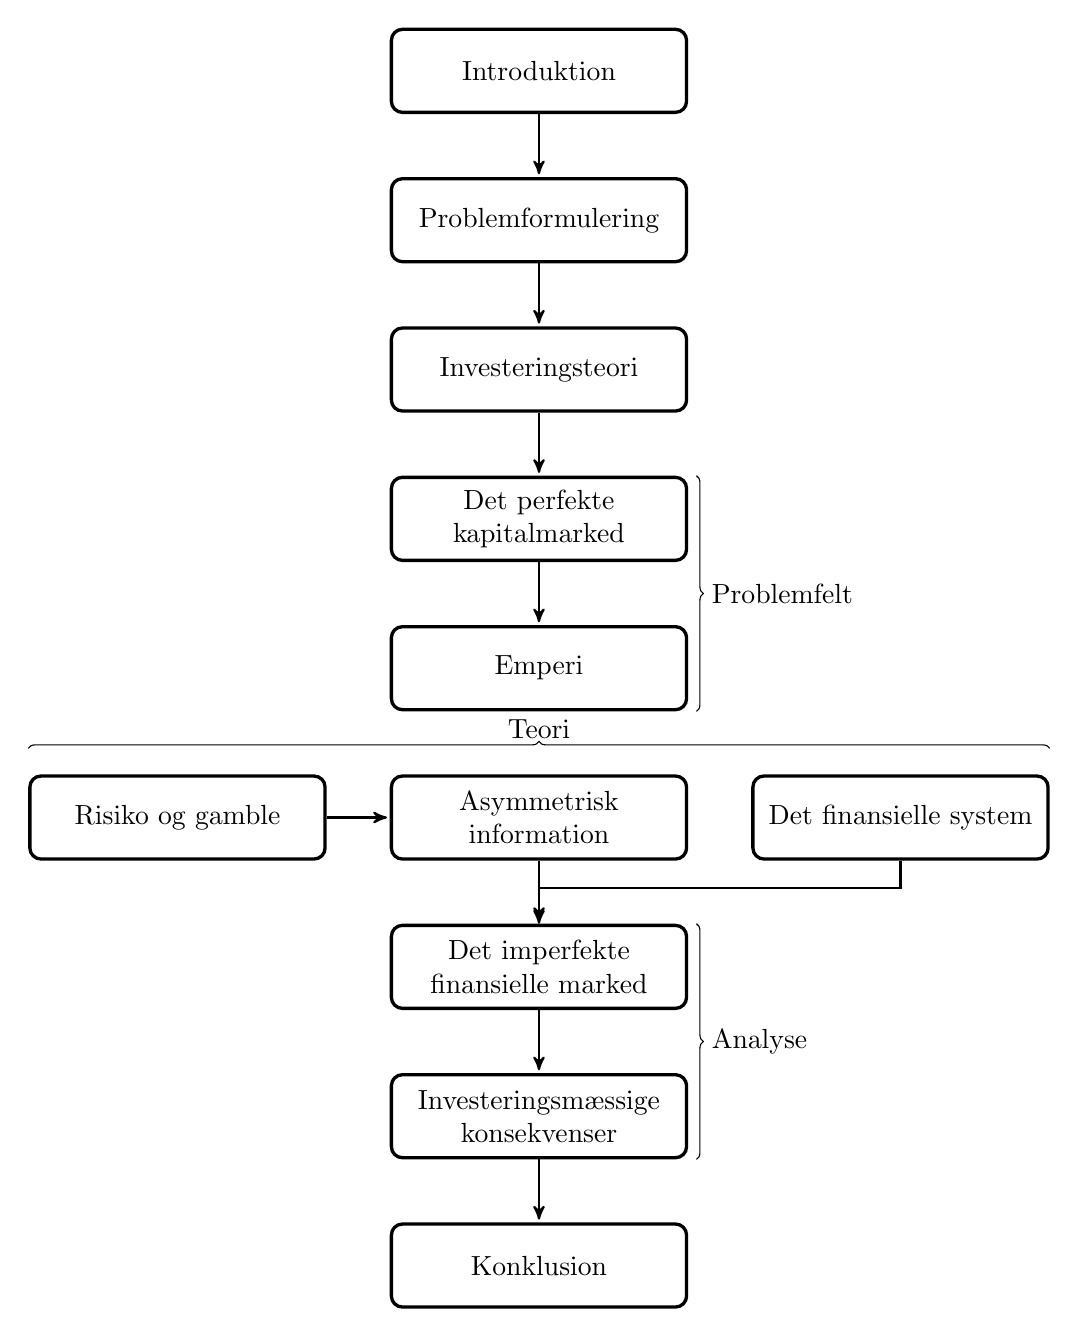
\begin{tikzpicture}
  [node distance=.8cm,
  start chain=going below,]
     \node[punktchain, join] (intro) {Introduktion};
     \node[punktchain, join] (probf)      {Problemformulering};
     \node[punktchain, join] (investeringer)      {Investeringsteori};
     \node[punktchain, join] (perfekt) {Det perfekte kapitalmarked};
     \node[punktchain, join, ] (emperi) {Emperi};
      \node (asym) [punktchain ]  {Asymmetrisk information};
      \begin{scope}[start branch=venstre,
        %We need to redefine the join-style to have the -> turn out right
        every join/.style={->, thick, shorten <=1pt}, ]
        \node[punktchain, on chain=going left, join=by {<-}]
            (risiko) {Risiko og gamble};
      \end{scope}
      \begin{scope}[start branch=hoejre,]
      \node (finans) [punktchain, on chain=going right] {Det finansielle system};
    \end{scope}
  \node[punktchain, join,] (disk) {Det imperfekte finansielle marked};
  \node[punktchain, join,] (makro) {Investeringsmæssige konsekvenser};
  \node[punktchain, join] (konk) {Konklusion};
  % Now that we have finished the main figure let us add some "after-drawings"
  %% First, let us connect (finans) with (disk). We want it to have
  %% square corners.
  \draw[|-,-|,->, thick,] (finans.south) |-+(0,-1em)-| (disk.north);
  % Now, let us add some braches. 
  %% No. 1
  \draw[tuborg] let
    \p1=(risiko.west), \p2=(finans.east) in
    ($(\x1,\y1+2.5em)$) -- ($(\x2,\y2+2.5em)$) node[above, midway]  {Teori};
  %% No. 2
  \draw[tuborg, decoration={brace}] let \p1=(disk.north), \p2=(makro.south) in
    ($(2, \y1)$) -- ($(2, \y2)$) node[tubnode] {Analyse};
  %% No. 3
  \draw[tuborg, decoration={brace}] let \p1=(perfekt.north), \p2=(emperi.south) in
    ($(2, \y1)$) -- ($(2, \y2)$) node[tubnode] {Problemfelt};
  \end{tikzpicture}
\end{document}
%%% Local Variables: 
%%% mode: latex
%%% TeX-master: t
%%% End: 
